\subsection{Chunked data streaming}

The Erlang NetInf NRS includes two different ways to stream chunked data. The first is the modified version of NetInf that removes the overhead of publishing each chunk to the NRS. The other implementation uses pure NetInf to publish each chunk. Both of them use an HTML5 interface to playback the stream. 

%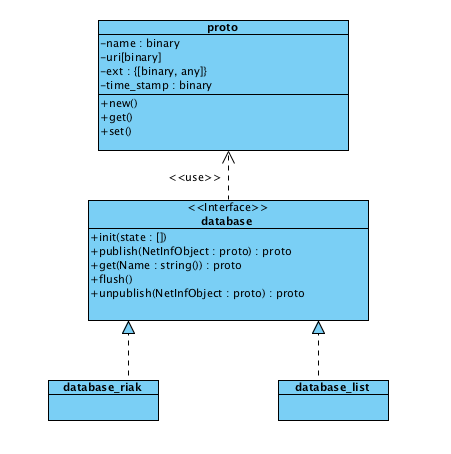
\includegraphics[scale=0.5]{./img/database_api.png}

\subsubsection{Content dispatcher}

To be able to transfer the chunks to the local HTML5 interface a content dispatcher service was added. The difference is that the content dispatcher service serves the NDOs' octects directly through HTTP, that is without the multi-part response as done in the HTTP CL. The module for this is the \textit{nn\_ct\_handler}. This service is spawned when the NRS system starts and runs on port 8078. To request the octects of the NDO \textit{ni:///sha-256-64;abc} pass the url:
\begin{verbatim}
http://localhost:8078/octets/ni%3A%2F%2F%2Fsha-256-64%3Babc 
\end{verbatim}

\subsubsection{Stream handler}
The stream handler module \textit{nn\_stream\_handler} handles fetching and polling of chunked octets between different NetInf nodes.
In both streaming implementations the logic for fetching the chunks is to shuffle the list of available locators and fetch all available chunks in the ICN. When there are no more chunks, the stream handler retries on a regular interval. After a defined number of retries it will finally terminate itself.  

\subsubsection{HTTP client handling}
The \textit{nn\_http\_client\_handler} module is used to serve the HTML5 interface for NetInf Get, Publish and Search requests. It forwards these requests to the local NRS. The client runs on port 8079. The different interfaces that can be seen are:

The interface for regular NetInf interaction, located at 
\textit{http://localhost:8079/}

The modified streaming, located at
\textit{http://localhost:8079/stream}

The pure streaming, located at
\textit{http://localhost:8079/streampure}

Other than the above viewable URIs there are a couple of other requests that are used to interact with the system. 

Subscribe to a modified chunked stream
\textit{http://localhost:8079/subscribe}

Subscribe to a pure NetInf stream
\textit{http://localhost:8079/subscribe/search\_and\_get}


\subsubsection{HTML5 interfaces}
To combine the video chunks, two HTML5 video elements are used to pre-cache the chunks through the content dispatcher. This is done by alternating the visibility and playback of the two elements with JavaScript. With this method of playback the video chunks looks like one continuous stream. 
To make the usability of the interface smoother, some asynchronous network request are used to communicate with the HTTP client.
To the right of the interface it is possible to see the current state of the local NRS. 

\subsubsection{Difference between implementations}
The main difference between the implementations is in the module \textit{nn\_event\_handler}. When requesting a chunk with the modified version, the special hash algorithm name \textit{demo} is used to avoid database lookups and content validation. To request chunk number 80 of the stream \textit{ni:///sha-256;abc}, the NDO name will be \textit{ni:///demo;abc80}. The metadata and locators in such a response are empty. To add a new chunk to the stream just increase the chunk number and add the physical chunk to the storage. 
\paragraph{The pure NetInf streaming} assumes that each chunk in the stream has been published to the NRS, with an ordinary NetInf publish request along with required metadata. The chunk metadata should include stream name and chunk number. For the stream \textit{mystream} and chunk number \textit{80} of \textit{ni:///sha-256;abc}, the metadata must include:
\begin{verbatim}
{"meta": {"stream":"mystream", "chunk":"mystream80"}}
\end{verbatim}
To obtain the chunk of a pure stream the receiver will have to search for each chunk and then get the NDO.

\subsubsection{Advantages and disadvantages}
The biggest advantage with the modified streaming is that the overhead of handling the chunks is reduced. A flaw is that the content validation has been disabled and it is possible to add chunks with modified content. 